% !TEX program = XeLaTeX
% !TEX encoding = UTF-8
\documentclass[UTF8,nofonts]{article}
%{ctexart}


%\setCJKmainfont[BoldFont=FandolSong-Bold.otf,ItalicFont=FandolKai-Regular.otf]{FandolSong-Regular.otf}
%\setCJKsansfont[BoldFont=FandolHei-Bold.otf]{FandolHei-Regular.otf}
%\setCJKmonofont{FandolFang-Regular.otf}

\usepackage{url}
\usepackage{cancel}
\usepackage{xspace}
\usepackage{graphicx}
\usepackage{multicol}
\usepackage{multirow}
\usepackage{subfig}
\usepackage{amsmath}
\usepackage{amssymb}
\usepackage[a4paper, width=186mm, top=18mm, bottom=18mm, includeheadfoot]{geometry}
%\usepackage[a4paper, width=140mm, top=18mm, bottom=22mm, includeheadfoot]{geometry}
\usepackage{booktabs}
\usepackage{array}
\usepackage{verbatim}
\usepackage{caption}
\usepackage{natbib}
\usepackage{booktabs}
\usepackage{float}
\usepackage{pdflscape}
\usepackage{mathtools}
\usepackage[usenames, dvipsnames]{xcolor}
\usepackage{afterpage}
\usepackage{pgf}
\usepackage{tikz}
\usepackage{dirtree}
\usepackage[spanish,mexico]{babel}
\usepackage[style=american]{csquotes}
\usepackage{amsfonts}
\usepackage{tikz}
\usepackage{tkz-graph}

\usetikzlibrary{arrows,decorations.pathmorphing,automata,positioning,backgrounds,fit,shapes.symbols,chains,intersections}

\newtheorem{definition}{Definición}[section]
\newtheorem{theorem}{Teorema}[section]
\newtheorem{lemma}{Lema}
\newtheorem{proof}{Prueba} [section]

\usepackage[toc, page, title, titletoc, header]{appendix}
\usepackage{marginnote}
\usepackage{tablefootnote}

%\renewcommand\appendixname{附\ 录}
%\renewcommand\appendixpagename{附\ 录}
%\renewcommand\appendixtocname{附\ 录}
\renewcommand\abstractname{Resumen}
\renewcommand{\figurename}{Figura}
\renewcommand\refname{Referencias}

\usepackage{perpage} %the perpage package
\MakePerPage{footnote} %the perpage package command

\usetikzlibrary{shapes.geometric}%
\usepackage{color}
%\usepackage[pages=some, placement=top]{background}
\usepackage{eso-pic}
\usepackage[final]{pdfpages}

%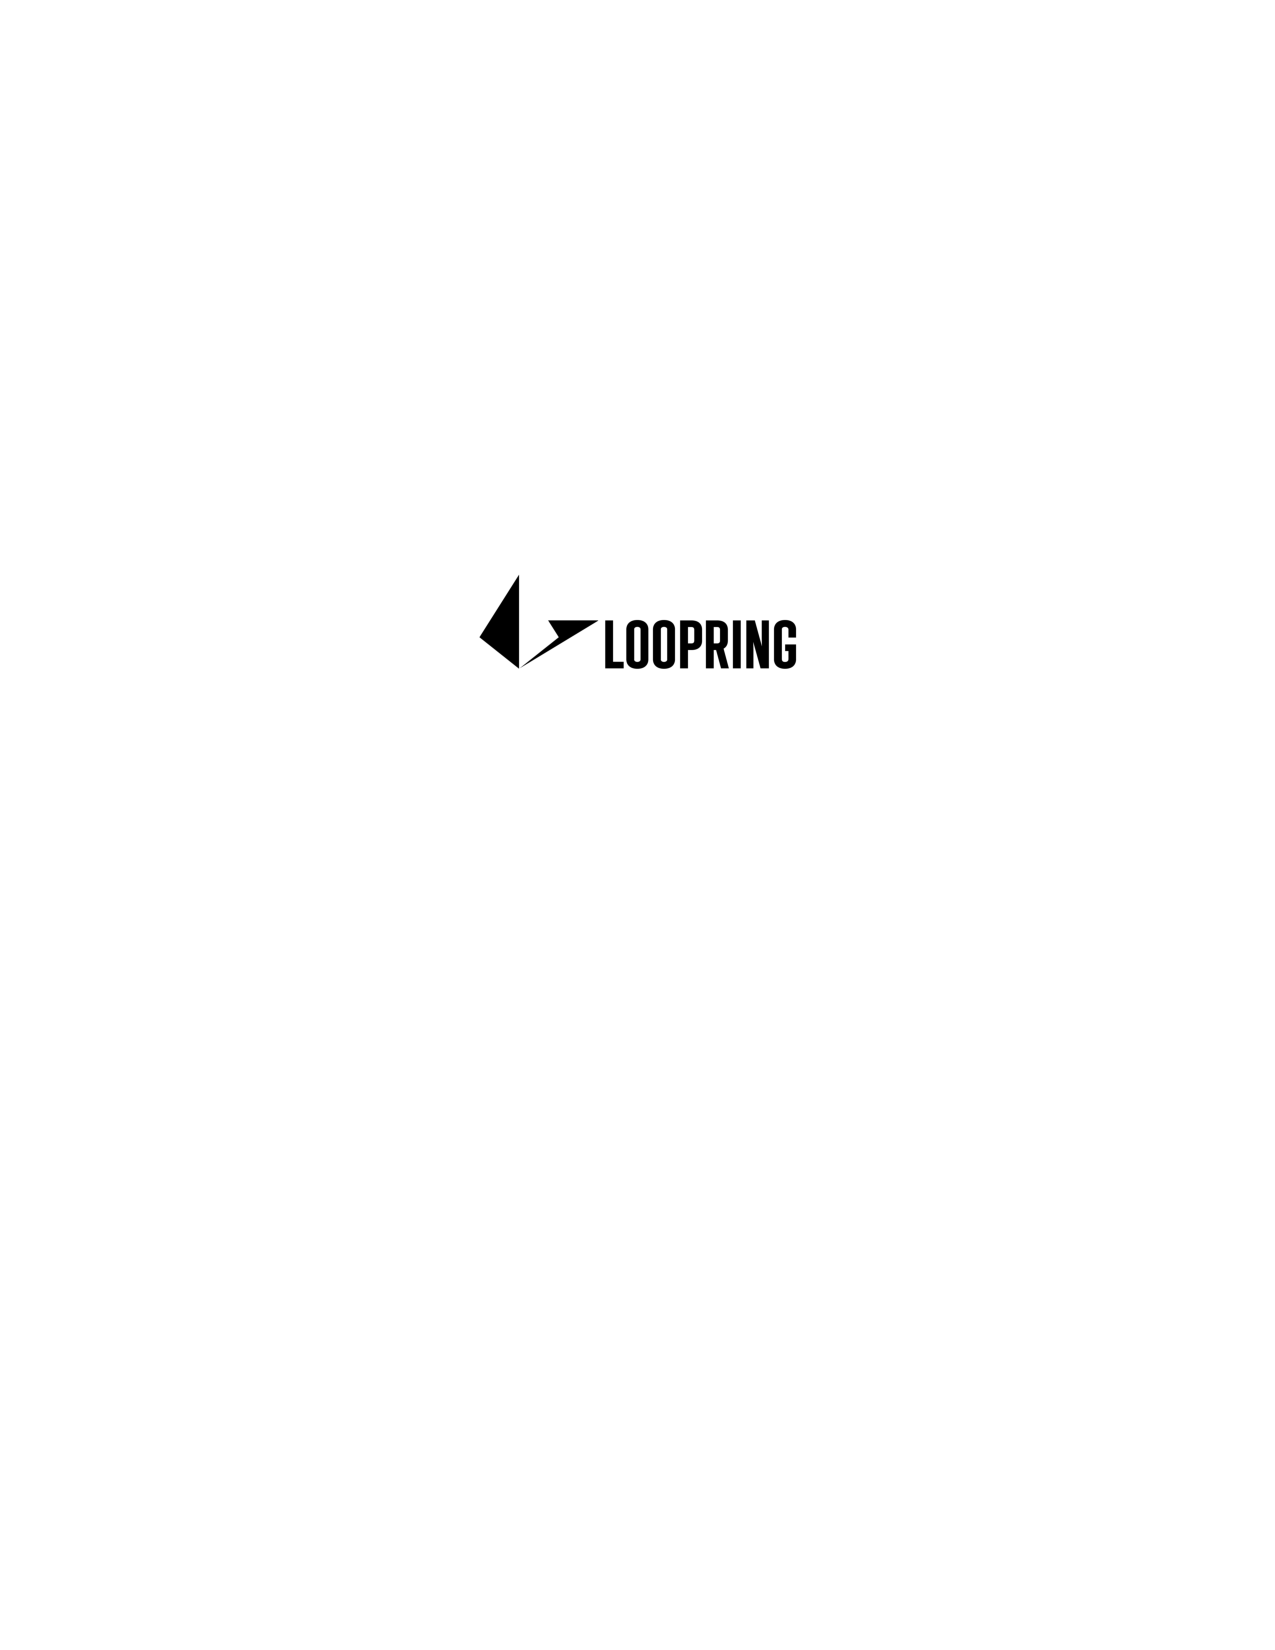
\includepdf[pages=1]{cover}
\hyphenpenalty=750

\title{\textbf{Loopring:}\\\textbf{Un protocolo de intercambio de \textit{tokens} descentralizado}}
\author{
  Daniel Wang\\
  \texttt{daniel@loopring.org}\\
  \and
  	Jay Zhou\\
  	\texttt{jay@loopring.org}\\
  	\and
  	Alex Wang\\
  	\texttt{alex@loopring.org}\\
  	\and
  	Matthew Finestone\\
  	\texttt{matt.finestone@gmail.com}\\ 
  \\
  \texttt{https://loopring.org}
 }

\makeatletter
\def\CTEX@section@format{\Large\bfseries}
\makeatother

\makeatletter
\newenvironment{tablehere}
 {\def\@captype{table}}
 {}

\newenvironment{figurehere}
 {\def\@captype{figure}}
 {}
\makeatother
%
%\newcommand\BackgroundPic{%
%\put(0, 0){%
%\parbox[b][\paperheight]{\paperwidth}{%
%\vfill
%\centering
%\includegraphics[width=\paperwidth, height=\paperheight, %
%%keepaspectratio]{images/background.jpg}%
%]{images/background.jpg}%
%\vfill
%}}}


\begin{document}
%\AddToShipoutPicture{\BackgroundPic}
\maketitle


\begin{abstract}
Loopring es un protocolo abierto para la creación de casas de cambio descentralizadas. Loopring opera como un conjunto público de contratos inteligentes responsables del intercambio y de la liquidación, con un grupo de agentes externos a la cadena de bloques añadiendo y comunicando órdenes. El protocolo es libre, extensible y sirve como un bloque de código estandarizado para aplicaciones descentralizadas (en inglés: \textit{decentralized applications} o \textit{dApps}) que incorporen la función de intercambio. Sus estándares interoperables facilitan el intercambio anónimo y libre de confianza en terceras partes. Una importante mejora frente a los protocolos de intercambio descentralizados actuales es su habilidad para mezclar y combinar diferentes órdenes entre sí, obviando las restricciones de uso de un único par de intercambio entre dos \textit{tokens}, y mejorando considerablemente la liquidez. Loopring también emplea una solución única y robusta para prevenir la inversión ventajista, o \textit{front-running}: el intento de enviar transacciones a un bloque antes que el proveedor de la solución original. Loopring es una tecnología agnóstica, por lo que puede lanzarse en cualquier cadena de bloques que admita contratos inteligentes. En el momento de redactarse este artículo, Loopring ya es operable en Ethereum \cite{buterin2017ethereum} \cite{wood2014ethereum} y Qtum \cite{dai2017smart}, y próximamente lo será en NEO \cite{atterlonn2018distributed}.
\end{abstract}



\begin{multicols}{2}
\section{Introducción\label{sec:introduction}}

Con la proliferación de activos basados en la cadena de bloques, la necesidad de intercambiar estos activos entre contrapartes ha aumentado considerablemente. A medida que miles de \textit{tokens} nuevos se van creando - incluyendo la conversión de activos tradicionales en \textit{tokens} - esta necesidad seguirá aumentando. Ya sea intercambiando \textit{tokens} por motivos especulativos, o bien digitalizando los activos para acceder a las redes mediante el uso de \textit{tokens} de utilidad nativos, la habilidad de intercambiar un criptoactivo por otro es fundamental para el ecosistema. En efecto, hay una energía potencial en los activos \cite{desotocapital}, y hacer efectiva esta energía - desbloqueando capital - requiere no sólo reivindicar la propiedad, que es lo que las cadenas de bloque han permitido indudablemente, sino también poder transferir y transformar estos activos libremente.
 
Por ello, el intercambio de \textit{tokens} (o valor) libre de confianza es un ejemplo convincente de la tecnología de la cadena de bloques. Hasta ahora, sin embargo, los entusiastas de las criptomonedas se han conformado mayormente con intercambiar \textit{tokens} en las casas de cambio centralizadas. El protocolo Loopring es necesario porque, tal como Bitcoin enfatizó responsablemente \cite{nakamoto2008bitcoin} en relación al dinero electrónico entre pares (en inglés: \textit{peer-to-peer}): \enquote{las principales ventajas se pierden si la confianza en una tercera parte es aún necesaria para evitar el doble gasto}. De la misma manera, las principales ventajas de los activos descentralizados se pierden si deben ser confiados y transferidos a través de casas de cambio centralizadas.

% format correction (Omar)
{\setlength{\parskip}{0cm}Intercambiar \textit{tokens} descentralizados en casas de cambio centralizadas no tiene sentido desde un punto de vista filosófico, puesto que falla en apoyar las virtudes que estos proyectos de descentralización defienden. Además, el uso de casas de cambio centralizadas presenta numerosos riesgos y limitaciones prácticas que se describen en la siguiente sección. Las casas de cambio descentralizadas (comúnmente referidas como DEX, del inglés: \textit{decentralized exchange}) \cite{schuh2015bitshares} \cite{bancor} \cite{kyber} han intentado hacer frente a estos problemas, consiguiendo en muchos casos disminuir los riesgos de seguridad mediante el uso de cadenas de bloques para la desintermediación. Sin embargo, todavía existe un margen de mejora considerable a medida que las DEX (gracias a sus capacidades) se conviertan en la infraestructura crucial para la nueva economía. Loopring, con su protocolo agnóstico y abierto para \textit{dApps}, pretende proveer a dicha infraestructura de las herramientas modulares necesarias.}



\section{Panorama actual de las casas de cambio\label{sec:current_exchange_landscape}}

\subsection{Insuficiencias de las casas de cambio centralizadas}
Los tres riesgos principales de las casas de cambio centralizadas son: 1) la falta de seguridad, 2) la falta de transparencia y 3) la falta de liquidez.

La \textbf{falta de seguridad} surge cuando los usuarios ceden el control de sus claves privadas (y por consiguiente, sus fondos) a una entidad central. Esto expone a los usuarios al riesgo de que las casas de cambio centralizadas caigan en manos de \textit{hackers} maliciosos. Los riesgos de seguridad y \textit{hackeo} a los que toda casa de cambio centralizada se expone son bien conocidos \cite{coincheckhack}  \cite{mcmillan2014inside}, y aun así comúnmente aceptados como un \enquote{riesgo implícito} del intercambio de criptomonedas. Las casas de cambio centralizadas continúan siendo una tentación para los \textit{hackers}, ya que sus servidores controlan millones de dólares en fondos de sus usuarios. Los desarrolladores de estas casas de cambio también pueden cometer errores accidentales y sin intencionalidad con dichos fondos. Simplemente, los usuarios no tienen el control de sus propios \textit{tokens} cuando estos son depositados en una casa de cambio centralizada.

La \textbf{falta de transparencia} expone a los usuarios al riesgo de que las casas de cambio descentralizadas deshonestas actúen injustamente. La diferencia aquí reside en las intenciones maliciosas de los operadores de estas casas de cambio. En las casas de cambio centralizadas, los usuarios no están intercambiando sus propios activos, sino un IOU (del inglés: \textit{I owe you}), un pagaré o instrumento de deuda informal. Cuando un \textit{token} es enviado a la cartera virtual de una casa de cambio, esta adquiere la custodia del mismo y ofrece un IOU en su lugar. Por tanto, todos los intercambios realizados dentro de la case de cambio son, a todos los efectos, entre los IOU de los usuarios. A la hora de realizar retiros, los usuarios canjean sus IOU con la casa de cambio, y reciben sus \textit{tokens} correspondientes en su dirección pública de monedero. Es a través de este proceso donde hay una falta de transparencia; una casa de cambio puede cerrar, congelar su cuenta, declararse en quiebra, etc. También es posible que usen los activos de los usuarios para otros propósitos mientras están en su custodia, como por ejemplo, para prestarlos a terceras partes. La falta de transparencia puede costar a los usuarios no solo una pérdida total de sus fondos, sino también impuestos de transacción más altos, retrasos durante máxima demanda, riesgo regulatorio y órdenes expuestas a inversión ventajista.

\textbf{Falta de liquidez.} Desde el punto de vista de los operadores de casas de cambio, la liquidez fragmentada impide la entrada de nuevas casas de cambio debido a dos escenarios de \enquote{ganador absoluto}. En primer lugar, la casa de cambio con el mayor número de pares de intercambio gana, debido a que los usuarios prefieren realizar todas sus operaciones en una sola casa de cambio. En segundo lugar, la casa de cambio con el libro de órdenes más grande gana, debido a que posee una horquilla de precios (comúnmente denominado en inglés como \textit{spread}) favorable para cada par de intercambio. Esto evita la competencia por parte de nuevas casas de cambio, debido a la dificultad para crear una liquidez inicial. Como resultado, muchas casas de cambio siguen poseyendo una cuota de mercado alta, a pesar de las quejas de sus usuarios e incluso de \textit{hackeos} importantes ocurridos en el pasado. Merece la pena apuntar que, a medida que una casa de cambio centralizada gane cuota de mercado, esta se convertirá en un objetivo mayor para los \textit{hackers}.

Desde el punto de vista de los usuarios, la liquidez fragmentada reduce considerablemente la experiencia del usuario. En una casa de cambio centralizada, los usuarios son capaces de comerciar únicamente dentro de los fondos de liquidez de la propia casa de cambio, con su propio libro de órdenes y entre los pares de intercambio a los que se da soporte. Para intercambiar el \textit{token} \verb|A| por el \textit{token} \verb|B|, los usuarios deben, o bien acudir a una casa de cambio que de soporte a ambos \textit{tokens}, o bien registrarse en diferentes casas de cambio, con la consiguiente divulgación adicional de información personal. A menudo, los usuarios necesitan realizar intercambios intermedios o iniciales, normalmente en BTC o ETH, pagando la horquilla correspondiente en el proceso. Además, el libro de órdenes puede no ser lo suficientemente grande como para completar un intercambio sin realizar deslizamiento (en inglés: \textit{slippage}). Incluso si la casa de cambio parece procesar un volumen grande, no hay garantía de que ese volumen y liquidez no sean falsos \cite{fakevolume}.

El resultado es un conjunto de silos de liquidez desconectados y un ecosistema fragmentado que se asemeja al antiguo sistema financiero, donde los volúmenes de cambio importantes se encuentran centralizados en unas pocas casas de cambio. Las promesas de liquidez global de la cadena de bloques no tienen ninguna virtud en las casas de cambio centralizadas.

\subsection{Insuficiencias de las casas de cambio descentralizadas}
Una de las diferencias entre las casas de cambio descentralizadas con respecto a las casas de cambio centralizadas es que los usuarios mantienen el control de sus claves privadas, y por tanto de sus activos, al realizarse los intercambios directamente en las cadenas de bloques subyacentes. Mediante el uso de la tecnología libre de confianza de las criptomonedas mismas, estas casas de cambio mitigan muchos de los riesgos de seguridad mencionados anteriormente. Sin embargo, los problemas relacionados con el rendimiento y las limitaciones estructurales todavía existen. 

La liquidez sigue siendo un problema frecuente, ya que los usuarios deben buscar contrapartes a través de fondos de liquidez y estándares dispersos. Los efectos de la liquidación fragmentada estarán presentes si la mayoría de las DEX o \textit{dApps} no se valen de estándares consistentes para operar entre sí, o si las órdenes no se comparten/envían a través de una red lo suficientemente amplia. La liquidez de los libros de órdenes limitadas, y especialmente su resiliencia -- cuán rápido se regeneran estas órdenes de precio límite -- puede afectar considerablemente a las estrategias de comercio \cite{limitorderliquidity}. La ausencia de estos estándares ha resultado no solo en una liquidez reducida, sino también en una exposición a una variedad de contratos inteligentes potencialmente inseguros.

Además, debido a que los intercambios se realizan en la cadena, las DEX heredan las limitaciones de la cadena de bloques subyacente, a saber: escalabilidad, retrasos en la ejecución (minado), y modificaciones de órdenes costosas. Debido a ello, los libros de órdenes en las cadenas de bloques no escalan especialmente bien, ya que la ejecución de código en la cadena de bloques incurre en un coste (gas), el cual hace que el coste de una cancelación múltiple de órdenes sea prohibitivo.

Finalmente, debido a que los libros de órdenes en las cadenas de bloques son públicos, la transacción para crear una orden es visible por los mineros mientras espera a ser minada en el siguiente bloque y añadida al libro de órdenes. Este retraso expone al usuario al riesgo de sufrir una inversión ventajista que mueva el precio en contra suya.

\subsection{Soluciones híbridas}
Debido a las razones anteriormente expuestas, las casas de cambio basadas estrictamente en la cadena de bloques presentan limitaciones que les impiden competir con las casas de cambio centralizadas. Hay una solución intermedia entre la libre confianza inherente a la cadena de bloques y la velocidad y flexibilidad de órdenes de una casa de cambio centralizada. Protocolos como Loopring y 0x \cite{warren20170x} ofrecen una solución intermedia de liquidación de intercambios dentro de la cadena con una gestión de órdenes fuera de la cadena. Estas soluciones giran en torno a contratos inteligentes abiertos, pero sortean ciertas limitaciones de escalabilidad ejecutando varias funciones fuera de la cadena y dando a los nodos flexibilidad en el cumplimiento de roles críticos para la red. Sin embargo, los inconvenientes de un modelo híbrido se mantienen \cite{costofdecent}. El protocolo Loopring propone, a través de este artículo, un enfoque de una solución híbrida con mejoras significativas.


\section{Protocolo Loopring\label{sec:loopring_protocol}}
Loopring no es una DEX, sino un protocolo modular para la creación de múltiples DEX en sus respectivas cadenas de bloques. Desensamblamos las partes que componen una casa de cambio tradicional para ofrecer, en su lugar, un conjunto público de contratos inteligentes y agentes descentralizados. Sus roles y funciones en la red son diversos, entre los que se incluyen: monederos, relés, una cadena de bloques de consorcio para la compartición de liquidez, exploración del libro de órdenes, mineros de anillos, y servicios de gestión de activos mediante \textit{tokens}. Debemos entender las órdenes de Loopring antes de definir cada uno de ellos.

\subsection{Anillo de órdenes\label{sec:order_ring}}
Las órdenes de Loopring se estructuran en lo que definimos como un modelo de orden unidireccional (MOU)\cite{coinport2014udom}. El MOU expresa las órdenes como peticiones de intercambio de \textit{tokens}, a un ratio \verb|amountS|/\verb|amountB|, (cantidad a vender/comprar)  en lugar de de los tradicionales precios de compra y venta (comúnmente referidos en inglés como \textit{bids and asks}). Como cada orden es simplemente un tipo de cambio entre dos \textit{tokens}, una característica potente del protocolo es la mezcla y combinación de múltiples órdenes en un intercambio circular. El uso de hasta 16 órdenes en lugar de un solo par de intercambio permite que haya un aumento drástico de la liquidez y la posibilidad de una mejora del tipo de cambio. 


\begin{center}
\begin{figurehere}
\centering
\tikzstyle{block} = [draw, fill=blue!20, rectangle, 
    minimum height=3em, minimum width=6em]
\tikzstyle{sum} = [draw, fill=blue!20, circle, node distance=1cm]
\tikzstyle{input} = [coordinate]
\tikzstyle{output} = [coordinate]
\tikzstyle{pinstyle} = [pin edge={to-,thin,black}]

\begin{tikzpicture}[
    auto, 
    node distance=2cm,
    >=latex',
    font=\bfseries\footnotesize\sffamily,
    order/.style={
		scale=0.7,
		rectangle,
		rounded corners,
		draw=black, 
		text centered,
%		text width=5cm,
		minimum height=12mm,
		fill=white
	},
	label/.style={
		scale=0.7
	}
  ]
    % We start by placing the blocks

  \node [order] (order2) 
 {%
 \begin{tabular}{l}
  \textbf{ORDEN\#2}\\
  \textbf{propietario: Y}\\
  \textbf{amountS: 9B}\\
  \textbf{amountB: 12C}
 \end{tabular}
 };
 
  \node [order, below of=order2, xshift=-3.5cm] (order1) 
 {%
 \begin{tabular}{l}
  \textbf{ORDEN\#1}\\
  \textbf{propietario: X}\\
  \textbf{amountS: 10000A}\\
  \textbf{amountB: 2B}
 \end{tabular}
 };
 
 
  \node [order, below of=order2, xshift=3.5cm] (order3) 
 {%
 \begin{tabular}{l}
  \textbf{ORDEN\#3}\\
  \textbf{propietario: Z}\\
  \textbf{amountS: 100C}\\
  \textbf{amountB: 160A}
 \end{tabular}
 };
 
 \draw [draw,->] (order1) -- node [label] {\textbf{7898A}} (order3);
 \draw [draw,->] (order2) -| node [label, xshift=-1.8cm] {\textbf{8B}} (order1);
 \draw [draw,->] (order3) |- node [label, xshift=1cm, yshift=0.24cm] {\textbf{98C}} (order2);

\end{tikzpicture}

\caption{Un anillo compuesto de 3 órdenes}
\label{fig:ring}
\end{figurehere}
\end{center}


La figura anterior muestra un anillo compuesto de 3 órdenes. Cada orden de venta de \verb|tokenS| es otra orden de compra de \verb|tokenB|. Esto crea un bucle que permite a cada orden intercambiar los \textit{tokens} deseados sin requerir de una orden opuesta para su par de \textit{tokens}. Las órdenes mediante pares de intercambio tradicionales aún pueden ser realizadas en lo que sería un caso especial de anillo de órdenes formado por tan solo 2 órdenes.

\begin{definition}[anillo de órdenes] Dados $n$ tokens distintos $C_{0}$, $C_{1}$, $\cdots$, $C_{n-1}$  y $n$ órdenes distintas $O_{0\rightarrow 1}$, $\cdots$, $O_{i\rightarrow i\oplus 1}$, $\cdots$, $O_{n-1 \rightarrow 0}$. Estas órdenes pueden formar un anillo de órdenes para el siguiente intercambio:
$$O_{0\rightarrow 1} \rightarrow \cdots \rightarrow O_{i\rightarrow i\oplus 1} \rightarrow \cdots \rightarrow O_{n-1\rightarrow 0} \text{, }$$
donde $n$ es la longitud del anillo, y $i\oplus 1 \equiv i+1 \mod n$.
\end{definition}

Un anillo de órdenes es válido cuando todas las transacciones que la componen pueden realizarse a un tipo de cambio igual o mejor que el valor original especificado implícitamente por el usuario. Para verificar la validez del anillo de órdenes, los contratos inteligentes del protocolo Loopring deben recibir, por parte de los mineros, anillos de órdenes cuyo producto del tipo de cambio original de todas las órdenes sea igual o mayor que 1.

En el siguiente ejemplo supondremos que Alicia y Bob quieren intercambiar sus \textit{tokens} \verb|A| y \verb|B|. Alicia tiene 15 \textit{tokens} \verb|A| y quiere 4 \textit{tokens} \verb|B| por ellos; Bob tiene 10 \textit{tokens} \verb|B|  y quiere 30 \textit{tokens} \verb|A| por ellos.

¿Quién de los dos está comprando y quién está vendiendo? Esto depende únicamente del activo en que nos basemos para determinar el precio. Si el \textit{token} \verb|A| es la referencia, entonces Alicia está comprando el \textit{token} \verb|B| a un precio de ${15 \over 4} = 3.75$\verb|A|, mientras que Bob está vendiendo 10 \textit{tokens} \verb|B| a un precio de ${30 \over 10} = 3.00$\verb|A|. En el caso de que escojamos el \textit{token} \verb|B| como referencia, diremos entonces que Alicia está vendiendo 15 \textit{tokens} \verb|A| a un precio de ${4\over 15}=0.26666667$\verb|B| y Bob está comprando 10 \textit{tokens} \verb|A| a un precio de ${10 \over 30}=0.33333334$\verb|B|. Distinguir entre el comprador y el vendedor es algo puramente arbitrario.

En el primer escenario, Alicia está dispuesta a pagar un precio más alto ($3.75$\verb|A|) que el precio de venta de los \textit{tokens} de Bob ($3.00$\verb|A|), mientras que en el segundo escenario Bob está dispuesto a pagar un precio más alto ($0.33333334$\verb|B|) que el precio de venta de los \textit{tokens} de Alicia ($0.26666667$\verb|B|). Queda claro que un intercambio es posible cuando el comprador está dispuesto a pagar un precio igual o más alto que el precio del vendedor.

\begin{equation}
{{15\over 4} \over {30\over 10}} = {{10\over 30} \over {4\over 15}}={15 \over 4} \cdot {10 \over 30} = 1.25 > 1
\end{equation}

Por consiguiente, para que un conjunto de $n$ órdenes pueda ejecutarse, de manera parcial o completa, es necesario saber si el producto de cada uno de los tipos de cambio de las órdenes de compra es mayor que 1. De ser así, todas las $n$ órdenes pueden ser ejecutadas parcial o completamente \cite{supersymmetry}.

Si introducimos una tercera parte, Charlie, tal que ahora Alicia quiere dar $x_1$ \textit{tokens} \verb|A| y recibir $y_1$ \textit{tokens} \verb|B|, Bob quiere dar $x_2$ \textit{tokens} \verb|B| y recibir $y_2$ \textit{tokens} \verb|C|, y Charlie quiere dar $x_3$ \textit{tokens} \verb|C| y recibir $y_3$ \textit{tokens} \verb|A|. Existen los \textit{tokens} necesarios, y el intercambio es posible si:

\begin{equation}
{{x_1 \cdot x_2 \cdot x_3 \over y_1 \cdot y_2 \cdot y_3} \geq 1}
\end{equation}

Véase la sección \ref{anatomy} para más detalles sobre las órdenes de Loopring.

\section{Participantes del ecosistema\label{sec:ecosystem}}
{\setlength{\parskip}{-1mm}%format correction Omar
Los siguientes participantes del ecosistema ofrecen de manera conjunta todas las funcionalidades que una casa de cambio centralizada puede ofrecer:}
\begin{itemize}

\item \textbf{Monederos}: Un servicio o interfaz común de monedero que permite a sus usuarios acceder a sus \textit{tokens} y enviar órdenes a la red de Loopring. Los monederos serán incentivados por crear órdenes mediante la compartición de comisiones con los mineros de anillos (véase la sección \ref{sec:token}). Con la creencia de que el futuro del intercambio tendrá lugar dentro de la seguridad de los monederos individuales de los usuarios, es crucial conectar estos fondos de liquidez  a través de nuestro protocolo.

\item \textbf{Cadena de bloques de consorcio para la compartición de liquidez/malla de relés}: Una malla de relés para la compartición de órdenes y liquidez. Cuando los nodos ejecutan el código de relé de Loopring, estos pueden unirse a redes existentes y compartir la liquidez con otros relés a través de una cadena de bloques de consorcio. Esta primera versión de la cadena de bloques de consorcio que estamos construyendo permite la compartición de órdenes casi en tiempo real (bloques de 1-2 segundos), y reduce el historial antiguo, permitiendo descargas más rápidas por parte de los nodos nuevos. Cabe destacar que los relés no necesitan unirse a este consorcio: pueden actuar de forma individual y  no compartir liquidez, o bien crear y gestionar su propia red de compartición de liquidez.

\item \textbf{Relés/mineros de anillos}: Los relés son nodos que reciben órdenes de los monederos o de la malla de relés, mantienen públicos los libros de órdenes e historial de intercambios, y, de manera opcional, transmiten órdenes a otros relés (vía un medio externo arbitrario) y/o mallas de relés. El minado de anillos de órdenes es una característica -- no un requisito -- de los relés. Esta es una aplicación computacionalmente intensiva y se realiza completamente fuera de la cadena. A los relés con la capacidad de minar estos anillos se les denomina \enquote{mineros de anillos}, los cuales crean anillos mediante la unión de órdenes dispersas. Los relés tienen libertad para (1) escoger cómo comunicarse entre ellos, (2) cómo crear los libros de órdenes y (3) qué algoritmo de minado usar para minar los anillos de órdenes.

\item \textbf{Contratos inteligentes del protocolo Loopring (CIPL)}: Un conjunto público y abierto de contratos inteligentes que comprueba los anillos de órdenes recibidos por los mineros, liquida las órdenes y transfiere los \textit{tokens} en nombre de los usuarios, recompensa a los mineros y monederos con las comisiones de transacción y transmite eventos. Los relés y exploradores de órdenes prestan atención a estos eventos para mantener sus libros de órdenes e historial de intercambios actualizados. 

\item \textbf{Servicios de gestión de activos mediante \textit{tokens} (SGAT)}: Una solución para aquellos activos que no pueden ser intercambiados directamente en  Loopring. Estos son servicios centralizados gestionados por compañías u organizaciones de confianza. Los usuarios depositan activos (reales, dinero fíat o \textit{tokens} de otras cadenas) y a cambio reciben \textit{tokens} que pueden ser canjeados por su depósito original en el futuro. Loopring no es un protocolo de intercambio entre cadenas (mientras no exista una solución adecuada para ello), pero el SGAT permite el intercambio de \textit{tokens} ERC20 (del inglés: \textit{Ethereum Request for Comments}) \cite{ERC20} por activos físicos o activos digitales de otras cadenas de bloques. 


\end{itemize}


\section{Proceso de intercambio\label{sec:process}}



\begin{enumerate} 

\item \textbf{Autorización del protocolo}: En la figura \ref{fig:process}, el usuario \verb|Y|, quien quiere cambiar sus \textit{tokens}, autoriza a los CIPL a gestionar una cantidad \verb|amountS| de \textit{tokens} \verb|B| para su venta. Esta autorización no congela los \textit{tokens} del usuario, quien sigue siendo libre de moverlos mientras la orden no se ejecute.

\item \textbf{Creación de la orden}: El tipo de cambio y el libro de órdenes para el par \textit{token}\verb|B|/\textit{token}\verb|C| es ofrecido por los relés u otros agentes conectados a la red (p. ej., los exploradores de libros de órdenes). El usuario \verb|Y| crea una orden (de precio límite) especificando el número de \textit{tokens} a intercambiar (\verb|amountS| y \verb|amountB|) junto con otros parámetros a través de la interfaz de monedero integrada. El usuario puede también añadir una cantidad de \textit{tokens} LRx como comisión para los mineros de anillos; una comisión mayor en LRx implica una mayor probabilidad de que los mineros procesen la orden más rápidamente. El \textit{hash} de la orden se firma con la clave privada del usuario \verb|Y|.

\item \textbf{Envío de la orden}: El monedero envía la orden y su firma a uno o más relés, quienes actualizan su libro de órdenes público. El protocolo no requiere que estos libros estén estructurados de una manera específica, como por ejemplo, en orden de llegada. Todo lo contrario: los relés tienen el poder de tomar sus propias decisiones al construir sus libros de órdenes.

\item \textbf{Compartición de la liquidez}: Los relés transmiten la orden a otros relés a través de un medio de comunicación arbitrario. Una vez más, hay una flexibilidad en la manera de definir cómo interactúan los nodos entre sí. Existe una malla de relés fija para la compartición de liquidez dentro de la cadena de bloques de consorcio con el fin de facilitar un cierto nivel de conectividad de la red. Esta malla de relés ha sido optimizada para ser inclusiva y rápida.

\item \textbf{Minado del anillo (combinación de órdenes)}: Los mineros de anillos intentan ejecutar las órdenes (parcial o completamente) igualando o mejorando el tipo de cambio mediante la mezcla y combinación de unas órdenes con otras. El minado de anillos es la principal razón por la que el protocolo es capaz de ofrecer alta liquidez en cualquier par de intercambio. Si el tipo de cambio al que la orden se ejecuta es mejor que la que especificó el usuario \verb|Y|, el margen es compartido entre todas las órdenes del anillo. Como recompensa, el minero del anillo puede elegir entre adjudicarse parte de ese margen y devolver la comisión por transacción en LRx al usuario, o sencillamente conservar dicha comisión en LRx.

\item \textbf{Verificación y liquidación}: El anillo de órdenes es recibido por los CIPL. Estos realizan múltiples comprobaciones para verificar los datos proporcionados por el minero del anillo y determinan si el anillo puede ser liquidado de manera parcial o completa, en función del ratio de liquidación de órdenes internas y los \textit{tokens} disponibles en los monederos de los usuarios. Si todas las comprobaciones tienen éxito, el contrato transfiere automáticamente los \textit{tokens} a los usuarios, cobra las comisiones a los monederos y paga al minero simultáneamente. Si el saldo del usuario \verb|Y| calculado por los CIPL es insuficiente, la orden será catalogada como reducida: una orden reducida volverá a su estado normal cuando se depositen fondos suficientes en la dirección correspondiente, a diferencia de una cancelación, que supone una operación manual y unilateral irreversible.

\end{enumerate}

\begin{center}
\begin{figurehere}
\centering
\tikzstyle{block} = [draw, fill=blue!20, rectangle, 
    minimum height=3em, minimum width=6em]
\tikzstyle{sum} = [draw, fill=blue!20, circle, node distance=1cm]
\tikzstyle{input} = [coordinate]
\tikzstyle{output} = [coordinate]
\tikzstyle{pinstyle} = [pin edge={to-,thin,black}]

\begin{tikzpicture}[
    auto, 
    scale=0.7,
    node distance=2cm,
    >=latex',
    font=\bfseries\footnotesize\sffamily,
    order/.style={
		rectangle,
		scale=0.7,
		rounded corners,
		draw=black, 
		text centered,
%		text width=5cm,
		minimum height=12mm,
		minimum width=30mm,
		fill=white
	},
	role/.style={
		circle,
		scale=0.7,
		draw=black, 
		text centered,
%		text width=5cm,
		minimum height=12mm,
		minimum width=12mm,
		fill=white
	},
	steps/.style={
		circle,
		scale=0.7,
		draw=black, 
		text centered,
%		text width=5cm,
%		minimum height=12mm,
%		minimum width=12mm,
		fill=black,
		text=white
	},
	account/.style={
		circle,
		scale=0.7,
		draw=black, 
		text centered,
%		text width=5cm,
		minimum height=16mm,
		minimum width=16mm,
		fill=white
	},
	label/.style={
	  scale=0.7
    }
  ]

 
 \node [role] (user1)  {usuario X};
 \node [role, below of=user1] (user2)  {usuario Y};
 \node [role, below of=user2] (user3)  {usuario Z};
 \node [role, below of=user3, fill=gray!20] (relay1)  {relé M};
 \node [role, below of=relay1, fill=gray!20] (relay2)  {relé N};

 
 \node [order, left of=user1, xshift=-1cm] (order1) 
 {%
 \begin{tabular}{l}
  \textbf{ORDEN 1}\\
  \textbf{propietario: X}\\
  \textbf{amountS: 10000 A}\\
  \textbf{amountB: 2 B}
 \end{tabular}
 };
 
 \draw [draw, ->]  (user1) -- (order1) [label]{};
 \draw [bend right,->] (order1) to node [auto, scale=0.7] {} (relay1);
 \draw [bend right,->] (order1) to node [auto, scale=0.7] {} (relay2);
% \draw [draw, ->]  (order1) |- (relay1) [label]{};
% \draw [draw, ->]  (order1) |- (relay2) [label]{};
 
 \node [order,left of=user2, xshift=-1.5cm] (order2) 
 {%
 \begin{tabular}{l}
  \textbf{ORDEN 2}\\
  \textbf{propietario: Y}\\
  \textbf{amountS: 9  B}\\
  \textbf{amountB: 12 C}
 \end{tabular}
 };
 \draw [draw, ->]  (user2) -- (order2) [label]{};
 \draw [bend right,->] (order2) to node [auto, scale=0.7] {} (relay1);
 \draw [bend right,->] (order2) to node [auto, scale=0.7] {} (relay2);
% \draw [draw, ->]  (order2) |- (relay1) [label]{};
% \draw [draw, ->]  (order2) |- (relay2) [label]{};
% 
\node [order, left of=user3, xshift=-2cm] (order3) 
 {%
 \begin{tabular}{l}
  \textbf{ORDEN 3}\\
  \textbf{propietario: Z}\\
  \textbf{amountS: 100 C}\\
  \textbf{amountB: 160 A}
 \end{tabular}
 };
 \draw [draw, ->]  (user3) -- (order3) [label]{};
 \draw [bend right,->] (order3) to node [auto, scale=0.7] {} (relay1);
 \draw [bend right,->] (order3) to node [auto, scale=0.7] {} (relay2);
% \draw [draw, ->]  (order3) |- (relay1) [label]{};
% \draw [draw, ->]  (order3) |- (relay2) [label]{};
 
% // The Ring
\node [order, 
yshift=-1.5cm,
xshift=-2.75cm,
below of=relay2,
fill=gray!10,
minimum width=4.2cm,
minimum height=5cm] (ring) {};


\node [order, dashed, below of=relay2,yshift=-0.2cm,xshift=-2.5cm] (order11) 
 {%
 \begin{tabular}{l}
  \textbf{ORDEN 1}\\
  \textbf{propietario: X}\\
  \textbf{amountS: 10000 A}\\
  \textbf{amountB: 2 B}
 \end{tabular}
 };
 \node [order, dashed,below of=order11,xshift=-0.25cm,yshift=0.7cm] (order21) 
 {%
 \begin{tabular}{l}
  \textbf{ORDEN 2}\\
  \textbf{propietario: Y}\\
  \textbf{amountS: 9  B}\\
  \textbf{amountB: 12 C}
 \end{tabular}
 };
\node [order, dashed,below of=order21,xshift=-0.25cm,yshift=0.7cm] (order31) 
 {%
 \begin{tabular}{l}
  \textbf{ORDEN 3}\\
  \textbf{propietario: Z}\\
  \textbf{amountS: 100 C}\\
  \textbf{amountB: 160 A}
 \end{tabular}
 };
 
 % // The blockchain
\node [
rectangle,
fill=gray!20, 
right of=user1,
yshift=-4.5cm,
xshift=0.1cm,
scale=0.7,
minimum width=3.2cm,
minimum height=15.6cm] (blockchain) {\parbox[b][15cm]{1.3cm}{cadena de bloques}};
% blockchain accounts
  \node [account, right of=user1, xshift=1cm] (account1)  {cuenta X};
  \node [account, right of=user2, xshift=1cm] (account2)  {cuenta Y};
  \node [account, right of=user3, xshift=1cm] (account3)  {cuenta Z};
  \node [account, right of=relay1, xshift=1cm] (account4)  {cuenta M};
  \node [account, right of=relay2, xshift=1cm] (account5)  {cuenta N};
  \node [account, double, below of=account5, yshift=-1.5cm] (psc)  {CIPL};
  
 \draw [draw, ->]  (user1) -- (account1) [label]{};
 \draw [draw, ->]  (user2) -- (account2) [label]{};
 \draw [draw, ->]  (user3) -- (account3) [label]{};
% \draw [draw, ->]  (relay1) -- (account4) [label]{};
% \draw [draw, ->]  (relay2) -- (account5) [label]{};
 \draw [draw, double, thick]  (relay1) to node [auto, scale=0.6] {liquidez compartida}  (relay2) [label]{};
% \draw [draw, ->]  (relay1) -- (ring) [label]{};
 \draw [draw, ->]  (relay2) to node [auto, scale=0.7, xshift=-2.5cm, yshift=0.3cm] {minado del anillo}  (ring) [label]{};
 \draw [draw, ->]  (ring) to node [auto, scale=0.6, yshift=0.4cm] {envío de anillo con la} (psc) [label]{};
 \draw [draw, ->]  (ring) to node [auto, scale=0.6] {función: submitRing} (psc) [label]{};
 
 \draw [bend left,->] (account1) to node [auto, scale=0.7] {\textbf{7898 A}} (account3);
 \draw [bend left,->] (account2) to node [auto, scale=0.7] {\textbf{8 B}} (account1);
 \draw [bend left,->] (account3) to node [auto, scale=0.7] {\textbf{98 C}} (account2);
 
 \draw [bend left,->, dashed] (account1) to node [auto, scale=0.7] {} (account5);
 \draw [bend left,->, dashed] (account2) to node [auto, scale=0.7] {} (account5);
 \draw [bend left,->, dashed] (account2) to node [auto, scale=0.7, xshift=0.7cm, yshift=0.5cm] {\textbf{Verificación y}} (account5);
 \draw [bend left,->, dashed] (account2) to node [auto, scale=0.7, xshift=0.7cm, yshift=0cm] {\textbf{liquidación}} (account5);  
  
% \draw [draw,->] (order1) -- node [label] {\textbf{7898 A}} (order3);
% \draw [draw,->] (order2) -| node [label, xshift=-1.8cm] {\textbf{8 B}} (order1);
% \draw [draw,->] (order3) |- node [label, xshift=1cm, yshift=0.24cm] {\textbf{98 C}} (order2);

\node [steps, right of=user2, xshift=-0.6cm] () {1};
\node [steps, left of=user2, xshift=0.8cm] () {2};
\node [steps, left of=relay2, xshift=0.3cm, yshift=1cm] () {3};
\node [steps, left of=relay1, xshift=3.3cm, yshift=-1.6cm] () {4};
\node [steps, below of=relay2, xshift=-0.2cm, yshift=0.4cm] () {5};
\node [steps, right of=account3, xshift=-0.6cm] (step5) {6};

% \draw [bend left,->, dashed] (account3) to node [auto, scale=0.7, yshift=-1.0cm] {\textbf{liquidación de}} (account5);
 \draw [bend right, ->]  (psc) to node [auto, scale=0.7, xshift=0.1cm, yshift=0.9cm] {comisión} (step5) [label]{};
 
\end{tikzpicture}

\caption{Proceso de intercambio con Loopring}
\label{fig:process}
\end{figurehere}
\end{center}





%
%\end{multicols}
%
%\begin{center}
%\begin{figurehere}
%\includegraphics[height=8cm]{images/en_protocol.png}
%\caption{Loopring Trading Process}
%\label{fig: Loopringrotocol}
%\end{figurehere}
%\end{center}
%
%\begin{multicols}{2}

\section{Flexibilidad operacional\label{sec:business_model}}
Cabe destacar de nuevo que el estándar abierto de Loopring ofrece a sus participantes flexibilidad a la hora de decidir cómo operar. Los agentes son libres de implementar nuevos modelos de negocios que ofrezcan valor añadido a sus usuarios, generando ingresos mediante comisiones de LRx con el volumen de cambio u otros sistemas a su elección. El ecosistema es modular, y ha sido diseñado para apoyar la participación de múltiples aplicaciones.


\subsection{Libro de órdenes\label{sec:order_book}}
Los relés pueden elegir de qué manera los libros de órdenes muestran y emparejan las órdenes de los usuarios. La primera implementación de nuestro propio libro de órdenes sigue un modelo extrabursátil u OTC (siglas del inglés  \textit{over-the-counter}), donde las órdenes de precio límite son clasificadas únicamente en función de su precio. La antigüedad de dichas órdenes (la fecha y hora de envío) no tiene ninguna relevancia en el libro de órdenes. Sin embargo, un relé tiene libertad para diseñar su libro de órdenes de una manera que imite el sistema de emparejamiento de una casa de cambio centralizada tradicional, en la cual las órdenes son clasificadas en función de su precio, pero respetando también su antigüedad.  Si un relé quiere ofrecer este formato de libro de órdenes, puede colaborar/integrarse con un monedero para que envíe las órdenes únicamente a este relé, quien será capaz de emparejar las órdenes en función de la antigüedad. Cualquier configuración es posible.

Mientras que otros protocolos de DEX a veces necesitan que los relés tengan sus propios fondos - por ejemplo saldos de \textit{tokens} iniciales para poder aceptar órdenes - los relés de Loopring únicamente necesitan encontrar órdenes que puedan combinarse o emparejarse entre sí para realizar un intercambio, y sin el requisito previo de disponer de algún \textit{token}.

\subsection{Compartición de liquidez\label{sec:liquidity_sharing}}
Los relés también tienen libertad de elegir cómo compartir la liquidez (u órdenes) unos con otros. Nuestra cadena de bloques de consorcio no es más que una de las soluciones para conseguirlo, y el ecosistema es libre de conectarse y comunicarse como desee. Además de unirse a una cadena de bloques de consorcio, los relés pueden crear y gestionar la suya propia, creando las reglas y/o recompensas que crean oportunas. También pueden optar por trabajar solos, como se ha descrito anteriormente en la implementación de monederos con funciones de antigüedad. Aunque la comunicación con otros relés y la conexión en red ofrecen ventajas evidentes, diferentes modelos de negocio con diseños interesantes de compartición de comisiones pueden presentar también sus propios méritos.


\section{Especificación del protocolo\label{sec:protocol}}

\subsection{Anatomía de una orden\label{anatomy}}
Una orden es un conjunto de datos que describen la intención del intercambio que el usuario quiere realizar. Una orden de Loopring se define mediante el modelo de orden unidireccional, o MOU, tal que así:

\begin{verbatim}
  message Order {
    address protocol;
    address owner;
    address tokenS;
    address tokenB;
    uint256 amountS;
    uint256 amountB;
    unit256 lrcFee
    unit256 validSince; // tiempo en UNIX
    unit256 validUntil; // tiempo en UNIX
    uint8   marginSplitPercentage;  // [1-100]
    bool    buyNoMoreThanAmountB;
    uint256 walletId;
    // dirección de la autoría doble
    address authAddr;
   	// v, r y s son partes de la firma
    uint8   v;       
    bytes32 r;
    bytes32 s;
    // clave privada de la autoría doble,
    // no se usa para calcular el "hash" de la orden,
    // y por ello NO está firmada.
    string  authKey;          
    uint256 nonce;
  }
\end{verbatim}


Para asegurar el origen de la orden, esta se firma con la clave privada del usuario y usando el \textit{hash} de sus parámetros, excluyendo  la dirección \verb|authAddr|. El parámetro \verb|authAddr| es utilizado para firmar los anillos que incluyan dicha orden, previniendo así una posible inversión ventajista o \textit{front-running} (véase la sección \ref{sec:dual_authoring} para más detalles). La firma está representada por los campos \verb|v|, \verb|r| y \verb|s|, y es enviada junto con el resto parámetros de la órden a través de la red. Esto garantiza que la orden permanezca inmutable durante su vida. Incluso si la orden nunca es modificada, el protocolo puede todavía calcular su estado actual basado en el saldo de su dirección, junto con otras variables.



El MOU no incluye un precio (el cual debe ser representado en coma flotante por definición): en su lugar usa la variable \verb|rate| o $r$, expresada como un ratio o tipo de cambio \verb|amountS|/\verb|amountB|. Este ratio no es un número en coma flotante, sino una expresión que solo será evaluada con otros números enteros sin firmar bajo demanda, con la finalidad de mantener todos los resultados intermedios sin firmar y así aumentar la precisión del cálculo. 

\subsubsection{Cantidades de compra}

Cuando un minero de anillo combina las órdenes para crear un anillo, es posible que estas se puedan ejecutar a un ratio mejor, permitiendo a los usuarios obtener más \verb|tokenB| que la cantidad \verb|amountB| especificada. Sin embargo, si la variable \verb|buyNoMoreThanAmountB| es fijada como \verb|True| (verdadero en \textit{booleano}), el protocolo se asegura de que los usuarios reciban como máximo la cantidad \verb|amountB| de \verb|tokenB|. De este modo, el parámetro \verb|buyNoMoreThantokenB| del MOU establece cuándo una orden debe considerarse como ejecutada. El parámetro \verb|buyNoMoreThantokenB| fija un límite bien en la cantidad \verb|amountS| o la cantidad \verb|amountB|, y permite a los usuarios establecer intercambios más granulares que con las órdenes de compra/venta tradicionales.

Por ejemplo, con unas cantidades \verb|amountS| = 10 y \verb|amountB| = 2, el tipo de cambio se define como $r$ = 10/2 = 5. Así, el usuario está dispuesto a vender 5 \verb|tokenS| por cada \verb|tokenB|. El minero del anillo consigue un tipo de cambio igual a 4 para el usuario, permitiéndole recibir 2.5 \verb|tokenB| en lugar de 2. Sin embargo, si el usuario solo quiere 2 \verb|tokenB| y establece el valor del parámetro \verb|buyNoMoreThanAmountB| como \verb|True|, los CIPL realizan el intercambio a un tipo de cambio de 4: el usuario vende 4 \verb|tokenS| por cada \verb|tokenB|, ahorrando así 2 \verb|tokenS|. Este ejemplo no tiene en cuenta las comisiones por minado (véase la sección \ref{sec:fee_model}).

En efecto, si usamos


\begin{verbatim}
	      Order(amountS,tokenS,
	            amountB,tokenB,
	            buyNoMoreThantokenB)
\end{verbatim}

para representar una orden de manera simplificada, y tomando como ejemplo el par ETH/USD en las casas de cambio tradicionales; un modelo de compra/venta tradicional puede representar la primera y tercera orden que se muestran a continuación, pero no las otras dos:

\begin{enumerate}
	\item Vender 10 ETH a un ratio de 300 USD/ETH. Esta orden puede expresarse como:

{\setlength{\parskip}{0cm}\verb|Order(10, ETH, 3000, USD, False)|.}
	\item Vender ETH a un ratio de 300 USD/ETH para obtener 3000 USD. Esta orden puede expresarse como: \verb|Order(10, ETH, 3000, USD, True)|.
	\item Comprar 10 ETH a un ratio de 300 USD/ETH, Esta orden puede expresarse como: \verb|Order(3000, USD, 10, ETH, True)|.
	\item Gastar 3000 USD para comprar tantos ETH como sea posible a un ratio de 300 USD/ETH, Esta orden puede expresarse como: \verb|Order(3000, USD, 10, ETH, False)|.
\end{enumerate}



\subsection{Verificación del anillo\label{sec:ring_verification}}

Los contratos inteligentes del protocolo Loopring no realizan cálculos de tipos de cambio o cantidades, pero deben recibir y verificar los resultados enviados por los mineros de anillos. Dichos cálculos los realizan los mineros fundamentalmente por dos razones: (1) el lenguaje de programación para los contratos inteligentes (p. ej., solidity \cite{dannen2017introducing} en Ethereum) no soporta matemáticas de números en coma flotante, en concreto $pow(x, 1/n)$ (calcular la raíz n de un número en coma flotante), y (2) es preferible que la computación se realice fuera de la cadena para reducir el coste computacional de la cadena de bloques.


\subsubsection{Comprobación de subanillos\label{sec:sub_ring_check}}
Este paso previene que los arbitrajistas obtengan injustamente todo el margen de un anillo de órdenes mediante la inserción de nuevas órdenes en él. Cuando un anillo de órdenes válido es encontrado por un minero de anillos, puede ser tentador añadir órdenes al anillo para absorber completamente el margen del usuario (descuento en los tipos de cambio). Tal como se ilustra a continuación en la figura \ref{fig:subring}, un cálculo meticuloso de $x1$, $y1$, $x2$ y $y2$ hará que el producto del tipo de cambio de todas las órdenes sea exactamente 1, eliminando así el descuento. 

\begin{center}
\begin{figurehere}
\centering
\tikzstyle{block} = [draw, fill=blue!20, rectangle, 
    minimum height=3em, minimum width=6em]
\tikzstyle{sum} = [draw, fill=blue!20, circle, node distance=1cm]
\tikzstyle{input} = [coordinate]
\tikzstyle{output} = [coordinate]
\tikzstyle{pinstyle} = [pin edge={to-,thin,black}]

\begin{tikzpicture}[
    auto, 
    node distance=2cm,
    >=latex',
    font=\bfseries\footnotesize\sffamily,
    order/.style={
		scale=0.7,
		rectangle,
		rounded corners,
		draw=black, 
		text centered,
%		text width=5cm,
		minimum height=12mm,
		fill=white
	},
	label/.style={
		scale=0.7
	}
  ]
    % We start by placing the blocks

  \node [order] (order2) 
 {%
 \begin{tabular}{l}
  \textbf{ORDEN 2}\\
  \textbf{propietario: Y}\\
  \textbf{amountS: 9B}\\
  \textbf{amountB: 12C}
 \end{tabular}
 };
 
  \node [order, below of=order2, xshift=-3.5cm] (order1) 
 {%
 \begin{tabular}{l}
  \textbf{ORDEN 1}\\
  \textbf{propietario: X}\\
  \textbf{amountS: 10000 A}\\
  \textbf{amountB: 2 B}
 \end{tabular}
 };
 
 
  \node [order, below of=order2, xshift=3.5cm] (order3) 
 {%
 \begin{tabular}{l}
  \textbf{ORDEN 3}\\
  \textbf{propietario: Z}\\
  \textbf{amountS: 100 C}\\
  \textbf{amountB: 160 A}
 \end{tabular}
 };
 
   \node [order, below of=order3, fill=gray!20] (order4) 
 {%
 \begin{tabular}{l}
  \textbf{ORDEN 4}\\
  \textbf{propietario: M}\\
  \textbf{amountS: x1 A}\\
  \textbf{amountB: y1 B}
 \end{tabular}
 };
 
 
  \node [order, below of=order1, fill=gray!20] (order5) 
 {%
 \begin{tabular}{l}
  \textbf{ORDEN 5}\\
  \textbf{propietario: M}\\
  \textbf{amountS: x2 C}\\
  \textbf{amountB: y2 A}
 \end{tabular}
 };
 
 \draw [draw,->] (order1) -- node [label, xshift=-2cm] {} (order5);
 \draw [draw,->] (order2) -| node [label, xshift=-1.6cm] {} (order1);
 \draw [draw,->] (order3) |- node [label, xshift=1cm] {} (order2);
 \draw [draw,->] (order4) -- node [label, xshift=1.8cm] {} (order3);
 \draw [draw,->] (order5) -- node [label, yshift=0.2cm] {} (order4);
  
\end{tikzpicture}

\caption{Un anillo de órdenes con un subanillo}
\label{fig:subring}
\end{figurehere}
\end{center}

Esto es una adición a la red de cero riesgo y cero valor, y se considera una conducta injusta por parte del minero del anillo. Con el fin de evitar esto, Loopring requiere que un bucle válido no contenga ningún subanillo. Para comprobar esto, los CIPL se aseguran de que un \textit{token} no puede estar en una posición de venta o de compra dos veces. En el diagrama superior se observa que el \textit{token} \verb|A| está definido como \textit{token} de compra y venta dos veces, lo cual no estaría permitido. 


\subsubsection{Comprobación del ratio de compleción\label{sec:fill_rate_check}}


Los cálculos de tipo de cambio en el anillo de órdenes son realizados por los mineros debido a las razones previamente expuestas. Son los CIPL los que deben verificar que sean correctos. Primero, se verifica que el ratio de compra por el que el minero del anillo puede realizar cada orden sea igual o menor que el ratio original establecido por el usuario. Esto asegura que dicho usuario obtiene un tipo de cambio igual o mejor que el que solicitó al realizar la transacción. Una vez los tipos de cambio se han confirmado, los CIPL se aseguran de que cada orden en el anillo de órdenes comparta el mismo descuento o ahorro del tipo de cambio. Por ejemplo, si el descuento sobre el tipo de cambio es $\gamma$, entonces el precio de cada orden será:

$r_{0\rightarrow 1} \cdot (1-\gamma)$, $r_{1\rightarrow 2} \cdot (1-\gamma)$, $r_{2 \rightarrow 0} \cdot (1-\gamma)$, esto cumple: 
\begin{equation}
r_{0\rightarrow 1} \cdot (1-\gamma)\cdot r_{1\rightarrow 2} \cdot (1-\gamma) \cdot r_{2 \rightarrow 0} \cdot (1-\gamma) = 1
\end{equation}
y por tanto: 
\begin{equation}
\gamma = 1- \frac{1}{\sqrt[3]{r_{0\rightarrow 1} \cdot r_{1\rightarrow 2} \cdot r_{2\rightarrow 0}}}\text{.}
\end{equation}
Si la transacción se realiza a través de $n$ órdenes, el \texttt{discount} será: 
\begin{equation}
\gamma = 1- \frac{1}{\sqrt[n]{\prod_{i=0}^{n-1} r^i}} \text{,}
\end{equation}

donde $r^i$ es el ratio de facturación de la $i$-ésima orden. Las órdenes pueden realizarse únicamente cuando el descuento es $\gamma \ge 0$; y el tipo de cambio actual de la la $i$-ésima orden ($O^i$) es $\hat{r^i} = r^i \cdot (1-\gamma)$, $\hat{r^i}\le r^i$.

Volviendo al ejemplo anterior donde Alicia tiene 15 \textit{tokens} \verb|A| y quiere 4 \textit{tokens} \verb|B| por ellos, Bob tiene 10 \textit{tokens} \verb|B| y quiere 30 \textit{tokens} \verb|A| por ellos. Si tomamos el \textit{token} \verb|A| como referencia, entonces Alicia está comprando los \textit{tokens} \verb|B| a un precio de $\frac{15}{4}$ = 3.75\verb|A|, mientras que Bob está vendiendo los \textit{tokens} \verb|B| a un precio de $\frac{30}{10}$ = 3.00\verb|A|. El descuento se calcula como: $\frac{150}{120}$ = 1.25, por tanto $\frac{1}{1.25}$ = 0.8 = $(1 −- \gamma)^2$. Como resultado, el tipo de cambio que hace que el intercambio sea equitativo para ambas partas es $\sqrt{0.8}$ $\cdot$ 3.75 $\approx$ 3.3541 \textit{tokens} \verb|A| por cada \textit{token} \verb|B|.

Bob da 4 \textit{tokens} \verb|B| y recibe 13.4164 \textit{tokens} \verb|A|, más de los 12 que esperaba por sus 4 \textit{tokens}. Alice recibe 4 \textit{tokens} \verb|B| como estaba previsto, pero da únicamente 13.4164 \textit{token} \verb|A| a cambio, menos de los 15 que estaba dispuesta a dar pos esos 4 \textit{tokens}.
Cabe destacar que una porción de este margen se destinará al pago de las comisiones para incentivar a los mineros y monederos (véase la sección \ref{sec:fee_model}).


\subsubsection{Seguimiento de la ejecución y cancelación}

Un usuario puede cancelar parcial o completamente una orden mediante el envío de una transacción especial a los CIPL, con detalles acerca de la orden y las cantidades a cancelar. Los CIPL reciben la información, almacenan las cantidades a cancelar y transmiten un evento de cancelación (\verb|OrderCancelled|) a la red. Los CIPL realizan un seguimiento de las cantidades completadas y canceladas mediante el almacenamiento de dichos valores usando el \textit{hash} de la orden como identificador. Estos datos son de acceso público y los eventos \verb|OrderCancelled| / \verb|OrderFilled| son transmitidos cuando se produce un cambio. El seguimiento de estos valores es crítico para los CIPL durante el proceso de liquidación de un anillo de órdenes.

Los CIPL también permiten cancelar todas las órdenes para cualquier par de \textit{tokens} con el evento \verb|OrdersCancelled| así como la cancelación de todas las órdenes para una dirección específica con el evento \verb|AllOrdersCancelled|.


\subsubsection{Escalado de órdenes\label{sec:order_scaling}}
Las órdenes son escaladas de acuerdo con el historial de cantidades canceladas y completadas y con el saldo actual de las cuentas emisoras. El proceso encuentra la orden con la menor cantidad pendiente para completar, según las características mencionadas previamente, y la usa como referencia para el escalado del resto de transacciones en el anillo de órdenes.


Encontrar la orden de menor valor puede ayudar a averiguar el volumen de ejecución para cada orden. Por ejemplo, si la $i$-ésima orden es la de menor valor, entonces el número de \textit{tokens} vendidos por cada orden $\hat{s}$ y el número de \textit{tokens} adquiridos por cada orden $\hat{b}$ puede calcularse como:

\[
\begin{split}
&\hat{s}^{i}=\overline{s}_i\text{, } \hat{b}^{i}=\hat{s}^{i}/ \hat{r}^i\text{, }\text{;}\\
&\hat{s}^{i\oplus 1}=\hat{b}^i\text{, } \hat{b}^{i\oplus 1}=\hat{s}^{i\oplus 1}/ \hat{r}^{i\oplus 1}\text{;}\\
&\hat{s}^{i\oplus 2}=\hat{b}^{i\oplus 1}\text{, } \hat{b}^{i\oplus 2}=\hat{s}^{i\oplus 2}/ \hat{r}^{i\oplus 2}\text{;}\\
& ...
%\text{.}
\end{split}
\]
donde $\overline{s}_i$ es el balance restante tras la ejecución parcial de las órdenes.

Durante la implementación, podemos asumir con seguridad que, sin importar cuál es la orden en el anillo de valor más bajo, solo se debería iterar un máximo de dos veces para calcular el volumen de ejecución de cada orden.

Por ejemplo: si la cantidad más pequeña de ejecución comparada con la orden original es de un 5\%, todas las transacciones en el anillo de órdenes serán reducidas a un 5\%. Una vez las transacciones se han completado, la orden que fue definida como la de menor cantidad de ejecución pendiente debería haber sido completada.

\subsection{Liquidación de un anillo\label{sec:settlement}}

Si un anillo de órdenes pasa todas las comprobaciones previamente descritas, dicho anillo puede completar sus transacciones y ser cerrado. Esto significa que todas las $n$ órdenes forman un anillo de órdenes cerrado, conectado como se muestra en la figura 4:

\begin{center}
\begin{figurehere}
\centering
\begin{tikzpicture}[
circle/.style={
		scale=0.75,
		rounded corners,
		draw=black, 
		text centered,
		}
]

\def \n {6}
\def \m {4}
\def \radius {1.4cm}
\def \margin {12} % margin in angles, depends on the radius

\foreach \s in {1,...,\m}
{
  \node[draw, circle] at ({360/\n * (\s - 1)}:\radius) {$O^\s$};
  \draw[<-, >=latex] ({360/\n * (\s - 1)+\margin}:\radius) 
    arc ({360/\n * (\s - 1)+\margin}:{360/\n * (\s)-\margin}:\radius);
}

\node[draw, circle] at ({360/\n * 4}:\radius) {$O^5$};
  \draw[<-, dashed, >=latex] ({360/\n * 4+\margin}:\radius) 
    arc ({360/\n * 4+\margin}:{360/\n * (5)-\margin}:\radius);
    
\node[draw, circle] at ({360/\n * 5}:\radius) {$O^n$};
  \draw[<-, >=latex] ({360/\n * 5+\margin}:\radius) 
    arc ({360/\n * 5+\margin}:{360/\n * (6)-\margin}:\radius);


\end{tikzpicture}
\caption{Liquidación de un anillo de órdenes}
\label{fig:settlement}
\end{figurehere}
\end{center}

El contrato inteligente \verb|TokenTransferDelegate| es usado por los CIPL para realizar las transacciones. La introducción de este delegado facilita la actualización del contrato inteligente del protocolo ya que ahora las órdenes solo necesitan autorizar a este delegado en lugar de a las diferentes versiones del protocolo.

Por cada orden en el anillo de órdenes se realiza un pago de \verb|tokenS| bien a la orden siguiente o a la orden previa, dependiendo de la implementación. Después se paga la comisión al minero del anillo en función del modelo de comisión escogido por dicho minero. Finalmente, se transmite el evento \verb|RingMined| una vez que todas las transacciones se han realizado.

\subsubsection{Eventos transmitidos\label{sec:events}}

El protocolo transmite eventos que permiten que los relés, los exploradores de órdenes y otros agentes reciban las actualizaciones del libro de órdenes de la manera más eficiente posible. Estos eventos transmitidos son:

\begin{itemize}
	\item \textbf{OrderCancelled}: Una orden en particular ha sido cancelada.
	\item \textbf{OrdersCancelled}: Todas las órdenes de un par de intercambio procedentes de una dirección de propietario han sido canceladas.
	\item \textbf{AllOrdersCancelled}: Todas las órdenes de todos los pares de intercambio procedentes de una dirección de propietario han sido canceladas.
	\item \textbf{RingMined}: Un anillo de órdenes ha sido liquidado con éxito. Este evento contiene datos relacionados con cada una de las transferencia internas del anillo.
\end{itemize}


\section{El \textit{token} LRx\label{sec:token}}
LRx es nuestra notación de \textit{token} generalizada. Por consiguiente, LRC es el \textit{token} de Loopring en Ethereum, LRQ en Qtum, LRN en NEO, etc. Otros tipos de \textit{token} LRx serán introducidos en el futuro a medida que el protocolo Loopring sea lanzado en otras cadenas de bloques públicas.

\subsection{Modelo de comisión\label{sec:fee_model}} 
Cuando un usuario crea una orden, este especifica la comisión en LRx a pagar al minero del anillo, junto con el porcentaje del posible margen (\verb|marginSplitPercentage|) que el minero puede reclamar. Esto se conoce como reparto del margen. La decisión de cuál escoger (comisión o parte del margen) corresponde al minero.

Una representación del reparto del margen sería:

\begin{center}
\begin{figurehere}
\centering
\begin{tikzpicture}[
scale=1,
font=\bfseries\footnotesize\sffamily,
classical/.style={thick,<->,shorten >=2pt,shorten <=2pt,>=stealth},
oneway/.style={->,dashed,shorten >=2pt,shorten <=2pt,>=stealth}
]
    % Draw axes
    \draw [->,thick] (0,1) node (yaxis) [above] {$$}
        |- (6.2,0) node (xaxis) [right] {$$};
        
    \draw
  	(4,0) coordinate (A)
  	(4,1) coordinate (A2)
  	(4.8,-0.6) coordinate (B)
  	(4.8,1) coordinate (B2)
  	(6,-0.6) coordinate (C)
  	(6,1) coordinate (C2);
  	
  	\fill [draw=none, fill=gray!20] 
    (4.8, 0) rectangle (6, 1);
    
  	\fill [draw=none, fill=gray!10] 
    (0, -0.6) rectangle (4.8, 0);

	\draw[thick] (0, -0.6) -- (0, 0.6) node[below]{$$};
  	\draw[thick, thin] (A) -- (A2) node[below]{$$};
  	\draw[thick, thin] (B) -- (B2) node[below]{$$};
  	\draw[thick] (C) node[below, xshift=0.5cm]{$Cantidad Compra Total$} -- (C2) ;
  	
  	\draw[classical] (0, 0.5) -> (4, 0.5) node[below]{$$};
  	\draw[classical] (4, 0.75) -> (4.8, 0.75) node[below]{$$};
%  	\draw[classical] (4.8, 0.5) -> (6, 0.5) node[below]{$$};
  	\draw[classical] (4, 0.25) -> (6, 0.25) node[below]{$$};

  	
  	\draw[oneway] (2, 1.2) node[above]{$Cantidad Compra Original$} -- (2, 0.5);
  	\draw[oneway] (4.4, 2.2) node[above]{$Cantidad Compra Adicional$} -- (4.4, 0.75);
  	\draw[oneway] (5.4, 1.6) node[above]{$Parte Margen$} -- (5.4, 1);
  	\draw[oneway] (5, -1.2) node[below]{$Margen$} -- (5, 0.25);
  	\draw[oneway] (2.4, -1.2) node[below]{$Cantidad Compra Actual$} -- (2.4, -0.5);



\end{tikzpicture}
\caption{Un reparto del margen del 60\%}
\label{fig:marginsplit}
\end{figurehere}
\end{center}

Si el margen en el anillo de órdenes es muy pequeño, el minero del anillo escogerá la comisión en LRx. Ahora bien, si el margen es lo suficientemente sustancial como para que el reparto merezca más la pena que la comisión en LRx, el minero escogerá el reparto del margen. Sin embargo, existe otra condición: cuando el minero del anillo escoge el reparto del margen, este debe pagar al usuario (creador de la orden) una comisión equivalente a los LRx que el usuario habría pagado al minero como comisión. Esto aumenta el umbral del precio por el que un minero aceptaría el reparto del margen al doble de la comisión en LRx de la orden, aumentando la tendencia a la elección de la comisión. Esto permite a los mineros de anillos recibir un ingreso constante en los anillos de órdenes con márgenes pequeños a cambio de recibir menos ingresos en los anillos de órdenes con márgenes altos. Nuestro modelo de comisiones está basado en la previsión de que a medida que el mercado crezca y madure, habrán cada vez menos anillos de órdenes con márgenes altos, y por tanto una necesidad de comisiones fijas en LRx como incentivo.


Esto lleva al siguiente gráfico:

\begin{center}
\begin{figurehere}
\centering
\begin{tikzpicture}[
font=\bfseries\footnotesize\sffamily,
oneway/.style={->,dashed,shorten >=2pt,shorten <=2pt,>=stealth},
scale=1]
    % Draw axes
    \draw [<->,thick] (0,2.7) node (yaxis) [above] {$y$}
        |- (5,0) node (xaxis) [right] {$x$};
        
    \draw
  	(1,1) coordinate (A)
  	(2,1) coordinate (B);
  	
  	
  	\draw[thick] (B) -- (3.7,2.7);
  	\draw[dotted] (B) -- (2,0) node[below] {$2f$};
  	\draw[dotted] (A) -- (1,0) node[below] {$f$};
  	\draw[thick,color=gray!70] (0,0) -- (2.7,2.7);
  	\draw[thick] (0,1) node[left] {$f$}--(B) node[     ]{$$};
 	\draw[oneway] (4,1) node[right]{$IngresosPorMinadoEsperados$} -- (3, 2);


\end{tikzpicture}
\caption{Modelo de comisiones de Loopring}
\label{fig:feemodel}
\end{figurehere}
\end{center}


donde $f$ es la comisión en LRx, $x$ es el reparto del margen e $y$ representa los ingresos por minado. La función $y=max(f, x-f)$ está indicada con una línea continua; si la comisión en LRx para esta orden es $0$, la función se convierte en $y=max(0, x - 0)$ que se reduce a $y=x$, tal como se indica en la línea gris.

Las consecuencias son:  
\begin{enumerate}
	\item Si el reparto del margen es 0, los mineros de anillos escogerán la comisión fija en LRx para seguir siendo incentivados. 
	\item Si la comisión fija en LRx es 0, la línea gris se cumple y los ingresos de los mineros de anillos estarán basados en un modelo lineal.
	\item Cuando el ingreso por reparto del margen sea mayor que  \textit{2x(comisión en LRx)}, los mineros de anillos escogerán el reparto del margen y pagarán al usuario en LRx.
\end{enumerate}

Cabe mencionar que si la comisión en LRx no es nula, siempre habrá una transferencia de LRx entre el minero del anillo y el emisor de la orden, independientemente de la opción que escoja el minero del anillo. O bien el minero obtiene su comisión en LRx, o bien paga la comisión en LRx de vuelta al emisor para obtener el reparto del margen en su lugar.

Los mineros de anillos compartirán cierto porcentaje de las comisiones con los monederos. Cuando un usuario coloca una orden a través de un monedero y esta se completa, el monedero es recompensado con una porción de las comisiones o del reparto del margen. Aunque esto es modular, y otros modelos de negocio o implementaciones únicas son posibles, nos decantamos por que los monederos reciban aproximadamente entre un 20\%-25\% de las comisiones obtenidas. Los monederos representan un objetivo primordial para la integración del protocolo Loopring, ya que son la base de los usuarios, pero tienen poca o ninguna fuente de ingresos.

\subsection{Gobernanza descentralizada}
En su esencia, el protocolo Loopring es un protocolo social en el sentido de que necesita de la cooperación y coordinación de sus miembros para operar efectivamente hacia un objetivo. Esto no es diferente de los protocolos criptoeconómicos en su conjunto, ya que su utilidad está protegida mayormente por los mismos mecanismos de coordinación de problemas \cite{vitalikgovernance}, equilibrio de la estrategia del gatillo y racionalidad limitada. Con este fin, los \textit{tokens} LRx no se usan únicamente para pagar comisiones, sino también para alinear los incentivos financieros de los diferentes participantes de la red. Dicho alineamiento es necesario para que cualquier protocolo consiga una mayor adopción, pero es particularmente crucial para un protocolo de intercambio, dado que su éxito depende mayormente de que se mejore la liquidez en un ecosistema descentralizado robusto.

Los \textit{tokens} LRx serán usados para realizar actualizaciones del protocolo a través de la gobernanza descentralizada. Los contratos inteligentes serán, en parte, gobernados por los poseedores de \textit{tokens} para ofrecer continuidad y seguridad, y atenuar los riesgos de desvío de liquidez a causa de incompatibilidades. Debido a que los contratos inteligentes no pueden ser alterados una vez han sido lanzados, hay un riesgo de que las \textit{dApps} o los usuarios finales continúen interactuando con versiones obsoletas y se excluyan a sí mismos de los contratos actualizados. La mejorabilidad es crucial para el éxito del protocolo, ya que debe adaptarse a las demandas del mercado y a las cadenas de bloques subyacentes. La gobernanza descentralizada por parte de los depositarios de LRx permitirá las actualizaciones de los contratos inteligentes sin perturbar a las \textit{dApps} o a los usuarios finales, o sin confiar excesivamente en la abstracción de los contratos inteligentes. Los \textit{tokens} LRx tendrán un suministro fijo, y en el caso de LRC, un porcentaje está congelado por parte de la fundación Loopring para fondos orientados a la comunidad \cite{LRCtokendoc}.

Sin embargo, los poseedores de \textit{tokens} LRx no son los únicos a considerar para manejar la dirección del protocolo: relés/mineros de anillos, monederos, desarrolladores y demás son una parte integral del ecosistema, y su voz debe ser oída. De hecho, dado que estos agentes no necesitan conservar ningún LRx para realizar sus respectivas funciones (las reservas iniciales de \textit{tokens} no son obligatorias, debido a que los creadores o sostenedores de mercado tradicionales no existen) debemos permitir métodos alternativos para que sus intereses también puedan ser respetados. Es más, un sistema de voto \enquote{simple} basado en \textit{tokens}, fuera y dentro de la cadena, es un bálsamo imperfecto para el desacuerdo, ya que una baja participación de votantes o una baja concentración de depositarios presenta riesgos. Por consiguiente, el objetivo es implementar un modelo de gobernanza que esté construido en capas, y descanse en un convencimiento común de que la norma ha de ser un proceso de toma de decisiones. Esto puede ser facilitado por instituciones de coordinación que ofrezcan avisos de distintos tipos de participantes, y quizá de puntos principales del protocolo ya preestablecidos. A medida que esto florezca, la función de la fundación Loopring como tal evolucionará de desarrolladora del protocolo a delegada del protocolo.

\section{Protecciones contra fraude y ataque}

\subsection{Prevención de la inversión ventajista\label{sec:dual_authoring}}

En las casas de cambio descentralizadas, la inversión ventajista ocurre cuando alguien intenta copiar la solución de intercambio de otro nodo y que esta sea minada antes que la transacción original que se encuentra pendiente en el fondo de transacciones o \textit{mempool}). Esto se puede conseguir especificando una comisión de transacción mayor (precio del gas). El método principal de inversión ventajista en Loopring (y cualquier otro protocolo que realiza emparejamiento de órdenes) es el hurto de órdenes (del inglés: \textit{order-filch}): cuando un inversor ventajista roba una o más órdenes de un anillo de órdenes pendiente de liquidación; en particular para Loopring: cuando un inversor ventajista roba un anillo de órdenes entero de una transacción pendiente.


Cuando una transacción \verb|submitRing| no está confirmada y se encuentra todavía en el fondo de transacciones pendientes, cualquiera puede identificarla fácilmente y reemplazar la dirección \verb|minerAddress| con su propia dirección (definida como \verb|filcherAddress|), para entonces firmar de nuevo el contenido de la transacción con  \verb|filcherAddress|, reemplazando así la firma del anillo de órdenes. El ladrón puede fijar un precio de gas mayor y enviar una nueva transacción a la espera de que los mineros de anillos escojan su transacción para el siguiente bloque en lugar de la transacción \verb|submitRing| original.


Las soluciones usadas hasta ahora presentaban importantes desventajas: requerían de más transacciones y por consiguiente costaban más gas a los mineros de anillos; costando también el doble de tiempo liquidar un anillo de órdenes. Nuestra nueva solución, la autoría doble \cite{dualauthor}, supone configurar dos niveles de autorización para las órdenes - una para su liquidación y otra para el minado del anillo.

El proceso de autoría doble se describe a continuación: 

\begin{enumerate}

	\item El programa del monedero generará una pareja de clave pública/privada aleatoria para cada orden, y añadirá esta pareja al \textit{snippet} JSON de la orden. Un método alternativo consiste en reemplazar la clave pública con una dirección derivada de la misma para reducir el número de bits. En este caso, usamos \verb|authAddr| para representar dicha dirección, y \verb|authKey| para representar la correspondiente clave privada \verb|authAddr|.

	\item Se calcula el \textit{hash} de la orden con todos sus campos (exceptuando \verb|r|, \verb|v|, \verb|s|, y \verb|authKey|), y se firma el \textit{hash} usando la clave privada del propietario (\verb|owner|) y no la clave \verb|authKey|.

	\item El monedero enviará la orden junto con la clave \verb|authKey| a los relés para el minado del anillo. Los mineros verificarán que \verb|authKey| y \verb|authAddr| están correctamente emparejadas y que la firma de la orden es válida con respecto a la dirección del \verb|owner|.

	\item Cuando un anillo de órdenes es identificado, el minero del anillo usará las claves \verb|authKey| de cada una de las órdenes para firmar el \textit{hash} del anillo, la dirección \verb|minerAddress| y todos los parámetros de minado. Si un anillo de órdenes contiene $n$ órdenes, habrán $n$ firmas con sus respectivas $n$ claves \verb|authKey|. Estas firmas son denominadas \verb|authSignature|. El minero del anillo también puede necesitar firmar el \textit{hash} del anillo junto con todos los parámetros de minado usando la clave privada de su dirección \verb|minerAddress|.

	\item El minero del anillo invoca la función \verb|submitRing| con todos sus parámetros, así como las firmas \verb|authSignature| extras. Fíjese que las claves \verb|authKey| NO son parte de la transacción interna de la cadena y por tanto permanecen desconocidas para el resto de las partes a excepción del minero del anillo.


	\item El protocolo Loopring ahora comparará cada firma \verb|authSignature| con su correspondiente dirección \verb|authAddr| para cada orden, y rechazará el anillo de órdenes si falta cualquiera de estas firmas \verb|authSignature| o alguna de ellas es inválida.
 
\end{enumerate}

El resultado ahora es que:

\begin{itemize}

	\item  La firma de la orden (con la clave privada de la dirección del \verb|owner|) garantiza que la orden no pueda ser modificada, incluyendo la dirección \verb|authAddr|.
	\item  La firma del minero del anillo (con la clave privada de la dirección \verb|minerAddress|), de ser proporcionada, garantiza que nadie pueda usar su identidad para minar un anillo de órdenes.
	\item  La firma \verb|authSignature| garantiza que el anillo de órdenes no pueda ser modificado, incluyendo la dirección \verb|minerAddress|, y que ninguna orden pueda ser robada.

\end{itemize}

La autoría doble previene el hurto de anillos y órdenes a la vez que asegura que la liquidación de anillos de órdenes pueda hacerse en una sola transacción. Además, la autoría doble ofrece la posibilidad de que los relés puedan compartir órdenes de dos maneras: mediante compartición equitativa o inicua. Por defecto, Loopring opera como un modelo extrabursátil y únicamente soporta órdenes de precio límite, lo que significa que la antigüedad de las órdenes es ignorada. Esto implica que realizar una inversión ventajista a una orden no tendrá un impacto en el precio real de la misma, pero sí que influirá en su ejecución.

\section{Otros ataques}

\subsection{Ataque Sybil o DOS}
Los usuarios maliciosos -- actuando como ellos mismos o con identidades falsas -- podrían enviar una gran cantidad de órdenes pequeñas con el fin de atacar a los nodos de Loopring. Sin embargo, ya que se permite a los nodos rechazar órdenes según su propio criterio -- el cual pueden ocultar o revelar -- la mayoría de estas órdenes serían rechazadas por no dar suficiente beneficio cuando sean emparejadas. No apreciamos una amenaza en este tipo de ataques facultando a los relés para decidir como manejan sus órdenes.

\subsection{Saldo insuficiente}
Los usuarios maliciosos podrían firmar y difundir órdenes cuyo valor no sea nulo, pero cuyo saldo en la dirección de monedero sí sea cero. Los nodos podrían observar y darse cuenta de que el balance actual de algunas órdenes es cero, actualizar el estado de dichas órdenes y descartarlas. Los nodos han de gastar tiempo para actualizar el estado de una orden, pero también pueden minimizar el esfuerzo, por ejemplo, con la creación de listas negras de direcciones, cancelando órdenes vinculadas a estas.

\section{Conclusiones}

El protocolo Loopring tiene la intención de ser una capa fundamental para el intercambio descentralizado. Conseguir esto tendrá unas repercusiones profundas en la manera que las personas intercambiarán activos y valores. El dinero, como una mercancía intermedia, facilita o reemplaza las casas de trueque y resuelve la doble coincidencia de deseos \cite{unenumerated2006} (del inglés: \textit{double coincidence of wants}), donde dos contrapartes deben desear exactamente el bien o servicio del otro. De manera similar, el protocolo Loopring pretende eliminar nuestra dependencia de la coincidencia de deseos en los pares de intercambio mediante el uso de los anillos de órdenes para consumar los intercambios de manera más fácil. Esto es significativo por cómo la sociedad y los mercados intercambian \textit{tokens}, activos tradicionales y más. De hecho, de la misma manera que las criptomonedas descentralizadas suponen una amenaza para el control de una nación sobre el dinero, un protocolo combinatorio que pueda emparejar agentes (consumidores/productores) a escala es una amenaza teórica para el concepto de dinero en sí mismo.

Entre las ventajas del protocolo se incluyen:

\begin{itemize}
	\item No se sacrifica rendimiento a costa de seguridad, ya que las órdenes se gestionan fuera de la cadena y la liquidación se realiza dentro de la misma.
	\item Mayor liquidez debido al minado de anillos y a la compartición de órdenes.
	\item La autoría doble resuelve el problema dañino de la inversión ventajista al que se enfrentan hoy en día las DEX y sus usuarios.
	\item Contratos inteligentes libres y públicos, que permiten a cualquier \textit{dApp} construir o interactuar con el protocolo.
	\item La estandarización entre operadores, lo cual permite mejoras en la red y la experiencia final de usuario
	\item Mantenimiento de una red flexible con respecto a la creación de libros de órdenes y a la comunicación.
	\item Barreras reducidas de entrada, que suponen menores costes de acceso a la red para los nodos y los usuarios finales.
	\item Intercambio anónimo directo desde los monederos de los usuarios.
\end{itemize}

\section{Agradecimientos}
Nos gustaría expresar nuestra gratitud a nuestros mentores, consejeros y a todas aquellas personas de la comunidad que han sido enormemente acogedoras y generosas a la hora de compartir sus conocimientos. En particular nos gustaría agradecer a: Shuo Bai (de ChinaLedger), el profesor Haibin Kan, Alex Cheng, Hongfei Da, Yin Cao, Xiaochuan Wu, Zhen Wang, Wei Yu, Nian Duan, Jun Xiao, Jiang Qian, Jiangxu Xiang, Yipeng Guo, Dahai Li, Kelvin Long, Huaxia Xia, Jun Ma y Encephalo Path por revisar y aportar sus valoraciones a este proyecto.


\bibliography{whitepaper}
\bibliographystyle{unsrt}


\end{multicols}

%
%\begin{appendices}
%
%\section{Loopring Implemented on EVM\label{app:protocol_ethereum}}
%
%\begin{center}
%\begin{figurehere}
%\centering
%\begin{tikzpicture}
%[node distance = 1cm, auto,font=\footnotesize,
%% STYLES
%every node/.style={node distance=3cm},
%% The comment style is used to describe the characteristics of each force
%comment/.style={rectangle, inner sep= 5pt, text width=4cm, node distance=0.25cm, font=\scriptsize\sffamily},
%% The force style is used to draw the forces' name
%force/.style={rectangle, draw, fill=black!10, inner sep=5pt, text width=4cm, text badly centered, minimum height=1.2cm, font=\bfseries\footnotesize\sffamily}] 
%
%% Draw forces
%\node [force] (impl) {LoopringProtocolImpl};
%\node [force, dashed, above of=impl] (protocol_interface) {LoopringProtocol};
%\node [force, left=1cm of impl] (nameregistry) {NameRegistry};
%\node [force, right=1cm of impl] (tokenregistry) {TokenRegistry};
%\node [force, below of=impl] (delegate) {TokenTransferDelegate};
%\node [force, left=1cm of delegate] (multisig) {TransferableMultsig};
%
%%%%%%%%%%%%%%%%
%% Change data from here
%
%% impl
%\node [comment, below=0.25 of impl] (comment-impl) {- Validates order-rings\\
%- Transfers tokens for settlement\\
%- Emits events};
%
%% nameregistry
%\node [comment, below=0.25cm of nameregistry]{- Registers wallets and relays};
%
%% protocol_interface
%\node [comment, below=0.25 of protocol_interface](comment-interface) {- Defines interfaces and events};
%
%% tokenregistry
%\node [comment, below=0.25 of tokenregistry] {- Registers ERC20/ERC223 tokens};
%
%% delegate
%\node [comment, below=0.25 of delegate] {- Transfers tokens on behalf of users};
%
%% PUBLIC POLICIES
%\node [comment, text width=3cm, below=0.25 of multisig] {- Enables multisignature ownership};
%
%%%%%%%%%%%%%%%%%
%
%% Draw the links between forces
%\path[->,thick] 
%(comment-interface) edge (impl)
%(nameregistry) edge (impl)
%(tokenregistry) edge (impl)
%(delegate) edge (comment-impl);
%
%\end{tikzpicture} 
%\caption{Smart Contracts}
%\label{fig:smartcontracts}
%\end{figurehere}
%\end{center}
%
%\section{Deployment}
%
%
%\subsection{Ethereum}
%The following smart contracts have been deployed on Ethereum mainnet:
%\begin{itemize}
%\item LRC: \verb|0xEF68e7C694F40c8202821eDF525dE3782458639f|
%\item TokenRegistry: \verb|0xa21c1f2AE7f721aE77b1204A4f0811c642638da9|
%\item TokenTransferDelegate: \verb|0x7b126ab811f278f288bf1d62d47334351dA20d1d|
%\item NameRegistry: \verb|0xd181c1808e3f010F0F0aABc6Fe1bcE2025DB7Bb7|
%\item LoopringProtocolImpl: \verb|0x0B48b747436f10c846696e889e66425e05CD740f|
%\end{itemize}
%
%\subsection{Qtum}
%The following smart contracts have been deployed on Qtum mainnet:
%\begin{itemize}
%\item LRQ: \verb| 2eb2a66afd4e465fb06d8b71f30fb1b93e18788d |
%\item TokenRegistry: \verb| c89ea34360258917daf3655f8bec5550923509b3 |
%\item TokenTransferDelegate: \verb| 60b3fa7f461664e4dafb621a36ac2722cc680f10 |
%\item NameRegistry: \verb| e26a27d92181069b25bc7283e03722f6ce7678bb |
%\item LoopringProtocolImpl: \verb| 5180bb56b696d16635abd8dc235e0ee432abf25d |
%\end{itemize}
%
%\end{appendices}
\end{document}
